\chapter{HASIL YANG DIHARAPKAN}

\section{Hasil yang Diharapkan dari Penelitian}

Dari penelitian yang akan dilakukan, diharapkan dapat dihasilkan sistem prediksi jumlah kalori yang terbakar saat berolahraga dengan treadmill dengan menggunakan kamera yang dapat memprediksi nilai jumlah kalori cukup baik dengan hasil perhitungan oleh treadmill.

\section{Hasil Pendahuluan}

Sampai saat ini, kami telah melakukan percobaan dalam tahap akuisisi data citra untuk menentukan posisi dan penentuan kamera dalam pengambilan gambar objek pada treadmill. Setelah itu dalam deteksi dan estimasi pose sudah dilakukan percobaan dengan menggunakan \emph{framework} MediaPipe dengan basis yang digunakan adalah \emph{body pose}. Hasil yang didapatkan dari proses percobaan deteksi dan estimasi pose adalah dapat dideteksi dan diestimasi pose tubuh menggunakan kamera \emph{webcam} secara \emph{realtime} dengan baik. Dengan dapat dilakukannya deteksi dan estimasi, dapat kemudian dipersiapkan untuk melakukan ekstrak fitur pose yang nantinya akan digunakan untuk proses \emph{training} dalam membuat model. Fitur yang telah dilakukan percobaan adalah dengan mengambil data gambar dari estimasi pose tubuh dengan warna dasar hitam dan diatur ulang untuk ukuran gambar menjadi persegi dan sama. Dengan begitu fitur yang telah dapat dilakukan ekstraksi tersebut akan dapat digunakan sebagai dataset yang nantinya akan dilakukan proses training dengan menggunakan \emph{Convolution Neural Network} (CNN) yang akan dilakukan pengerjaannya pada jadwal berikutnya. Hasil dari percobaan berupa kumpulan data gambar yang akan digunakan dalam proses penelitian terdapat pada Gambar \ref{fig:Dataset}. Kemudian hasil dari percobaan dalam melakukan deteksi dan estimasi pose lalu ekstrak fitur pose terdapat pada Gambar \ref{fig:EstimasiEkstrak}.

% Contoh input gambar dengan format *.jpg
\begin{figure} [ht] \centering
    % Nama dari file gambar yang diinputkan
    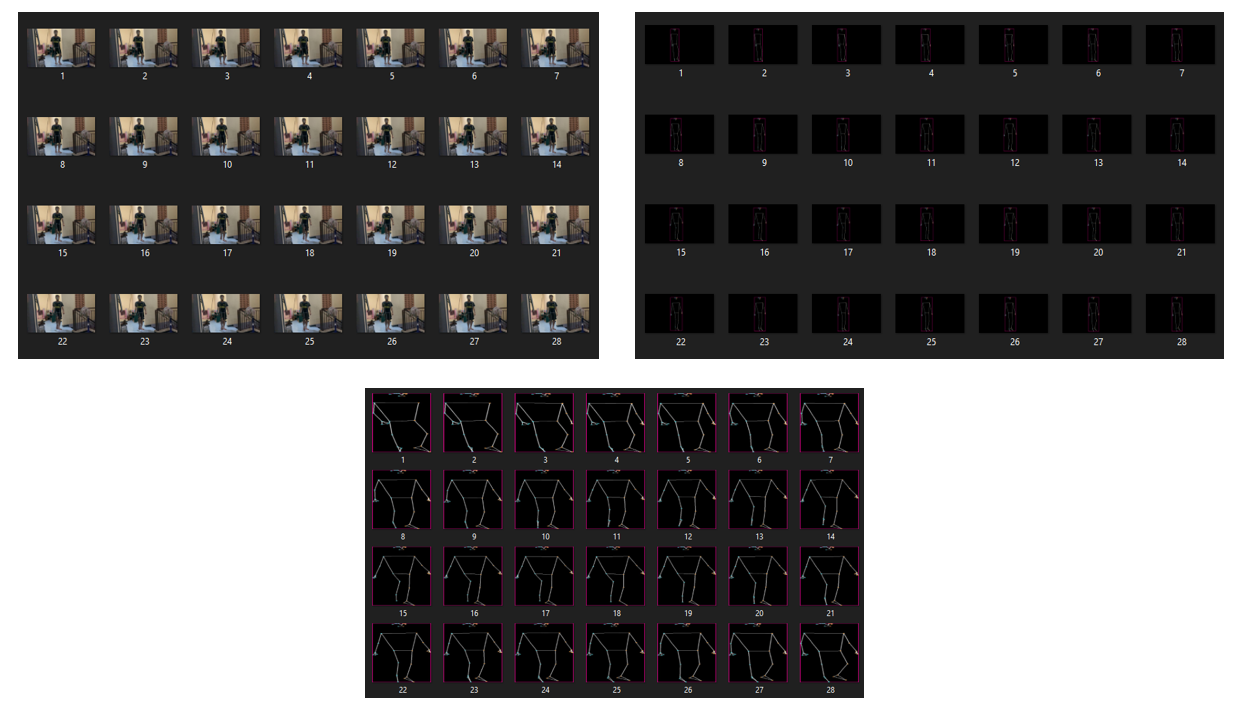
\includegraphics[scale=0.48]{gambar/dataset.png}
    % Keterangan gambar yang diinputkan
    \caption{Data gambar percobaan}
    % Label referensi dari gambar yang diinputkan
    \label{fig:Dataset}
\end{figure}

% Contoh input gambar dengan format *.jpg
\begin{figure} [ht] \centering
    % Nama dari file gambar yang diinputkan
    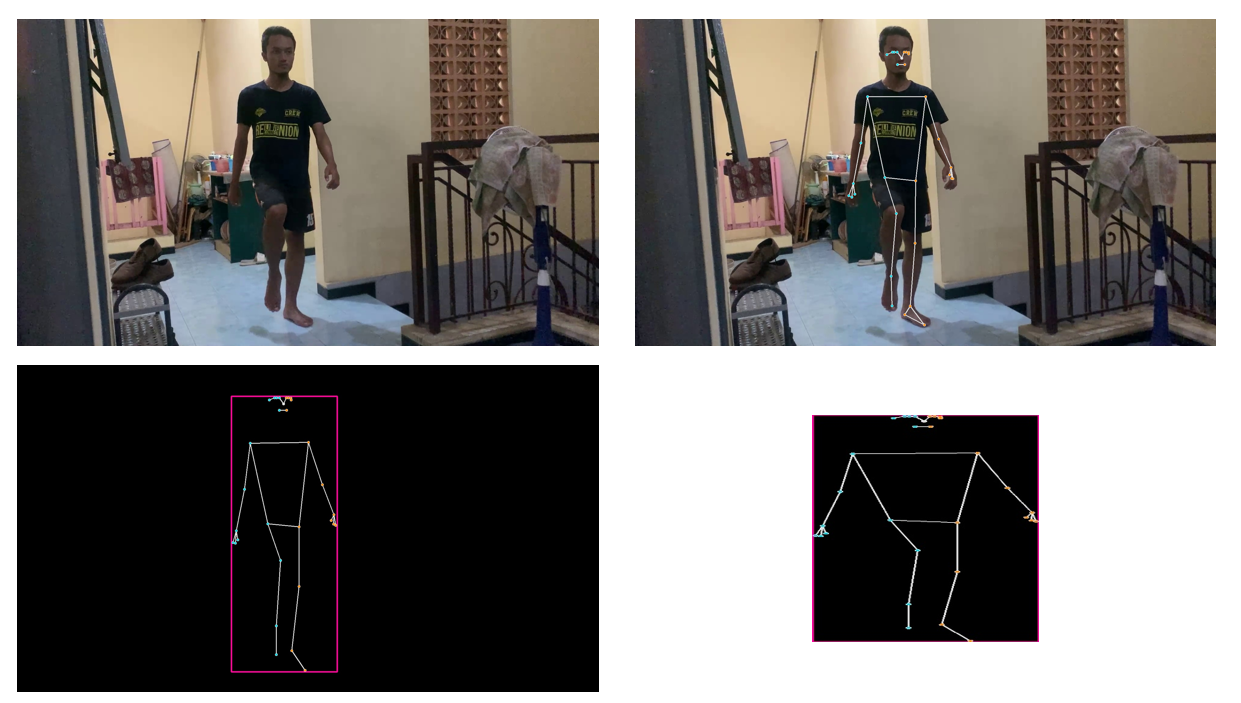
\includegraphics[scale=0.48]{gambar/estimasi ekstrak.png}
    % Keterangan gambar yang diinputkan
    \caption{Percobaan estimasi pose dan ekstrak fitur}
    % Label referensi dari gambar yang diinputkan
    \label{fig:EstimasiEkstrak}
\end{figure}
